%%% Local Variables: 
%%% mode: xelatex
%%% TeX-master: t
%%% End: 
 
%\documentclass[a4paper,10pt]{scrreprt}
%\documentclass[a4paper,10pt]{article}
%\documentclass[a4paper,10pt]{report}

\documentclass[unicode, 12pt, a4paper,oneside,fleqn]{article}
\usepackage[cm-default]{fontspec}
\defaultfontfeatures{Mapping=tex-text}    %% устанавливаем поведение шрифтов по умолчанию
\usepackage{polyglossia}    %% подключаем пакет многоязыкой верстки
%\setdefaultlanguage{russian}    %% установка языка по умолчанию
\setdefaultlanguage{english}    %% установка языка по умолчанию
%\setotherlanguages{english}
\setmainfont{Old Standard}      %% зададим основной шрифт документа
%\setmainfont{DejaVu Sans Mono}
\setmonofont{DejaVu Sans Mono}

\usepackage{mathtext}               % если нужны русские буквы в формулах
%\usepackage{ucs}
%\usepackage[utf8x]{inputenc}       % Кодировка входного документа;
                                   % при необходимости, вместо cp1251
                                   % можно указать cp866 (Alt-кодировка
                                   % DOS) или koi8-r.

\usepackage{textcomp}              % типографские значки

% \usepackage[T2A]{fontenc}           % Кодировка для шрифтов LH
%\usepackage{indentfirst}    % неизвестно
%\usepackage{cmap}           % неизвестно
%\usepackage[english,russian]{babel} % Включение русификации, русских и
                                    % английских стилей и переносов

%\renewcommand{\rmdefault}{ost_____} % add new font  Old_Standard
%\renewcommand{\sfdefault}{ost_____}
%\renewcommand{\ttdefault}{osti____}

\usepackage{graphics}
\usepackage{pgf}
\usepackage{wrapfig}
\usepackage{multicol}
\usepackage{multirow}
\usepackage{tabularx}
%\usepackage{fullpage}
%\usepackage{amsmath} % для спец знаков в формулах
%\usepackage{amssymb} % для спец знаков в формулах
\usepackage{topcapt} % подписи к таблицам
\usepackage{dcolumn} % выравнивание чисел
\usepackage{ulem} % подчёркивание

\hyphenpenalty=10000 % запретить переносы
%\tolerance-1 
\pretolerance10000 


\usepackage[colorlinks=true]{hyperref} % url hyperlink

\usepackage{makeidx} % индекс

%\newfontfamily\cyrillicfont{DejaVu Sans Mono}
%\newfontfamily{\cyrillicfont}{Liberation Mono}
\usepackage{verbatim} % печать неформатированного текста



\usepackage{listings} % печать исходного кода
%\lstloadlanguages{lisp}
\lstset{
  language=Pascal,
%  extendedchars=true, %Чтобы русские буквы в комментариях были 
  texcl,  %Чтобы русские буквы в комментариях были не слипшимися
  escapechar=|,
  frame=single,
  commentstyle=\itshape,
  inputencoding=utf8x,
  stringstyle=\bfseries
}



% вращение 
\usepackage{lscape}     % for %\begin{landscape} ...   %\end{landscape}
\usepackage{rotating}   % for sideways and \rotatebox{-90}{}




\author{Р.В.~Приходченко}
\title{поиск пути}
\frenchspacing


\makeindex

\begin{document}


\newcolumntype{Y}{>{\centering\arraybackslash}X}
%\newcolumntype{R}{>{\raggedleft\arraybackslash}X}


\maketitle
\tableofcontents


\begin{table}[ht]
  \begin{tabular}{cc}
    
\includegraphics[width=2cm]{../CC_BY-SA_88x31.png} &
    \shortstack{руководство распространяется в соответствии с
      условиями\\
      \href{http://creativecommons.org/licenses/by-sa/3.0/}{Attribution-ShareAlike} \\
      (Атрибуция — С сохранением условий) CC BY-SA \\
      Копирование и распространение приветствуется.}
  \end{tabular}
\end{table}

\section{Задача}
 Поиск пути.

  Возьмём идею которая была предложена мной в проекте
  расшифровки спектров полученных фотографированием интерферометра
  Фабри-Перо. Предположим что изображение содержит окружность
  (например белые точки - фон, чёрные - объекты в данном случае
  окружности). Через три точки на плоскости можно построить только
  одну окружность. Взяв любые три чёрные точки из изображения и находим
  центр $(x_i \  y_i)$ окружности которая бы проходила через эти три
  точки. Изображение состоит из множества чёрных точек, поэтому для
  большей точности можно (необязательно) повторить поиск центра для
  всех возможных комбинаций чёрных точек из изображения. Некоторая
  функция (среднее, медиана, ...) от полученного набора координат и
  будет наиболее приближена к реальному центру окружности.

  Упрощённый метод: Предположим что камера (из оптического сенсора
  мыши) вместе с линзой охватывают только область под роботом. Линии
  имеют радиус закругления больше чем размер область обзора камеры.
  Чем дальше находятся точки друг от друга тем больше точность (если
  взять координаты соседних чёрных пикселей то они скорее всего дадут
  неверные координаты центра круга). Возьмём координаты точек входа
  "A" и выхода "B" окружности из кадра (окружность больше обзора
  камеры и не поместилась в кадр целиком). проведём прямую между "A" и
  "B" и из центра опустим перпендикуляр. Ближайшую к перпендикуляру
  чёрную точку назовём "C". Комбинация точек (A, B, C) позволит найти
  центр окружности.

  Сложности:
\begin{enumerate}
\item точек входа (выхода) может быть несколько "A" и рядом с ней ещё
  одна "A" (линия отображается линзой на несколько пикселей) - это не
  страшно, ведь линия широкая и робот не выйдет за границы, но
  возможно он выберет не оптимальный путь (ошибка ~2cm - ширина линии)
  и проедет не по внутреннему а по наружному краю при повороте, что
  добавит дополнительные секунды к общему времени.

\item точки типа "d" на краю изображения затруднят поиск точек входа и
  выхода окружности.
  
  решение: обрезаем края изображения и повторяем поиск точек входа и
  выхода

\item аналогично, артефакты типа "e" которые окажутся близко к
  перпендикуляру.
  
  плохое решение: запоминаем предыдущие координаты центра. и если
  новые координаты центра будут очень далеко то это точка "e", а не
  точка "C". ищем новую точку. а плохое оно потому, что если линия
  представляет собой букву "S" то при переходе от нижнего полукруга к
  верхнему центр окружности перескочит на большое расстояние.

  хорошее решение?

\item места пересечения линии с собой "f".

  ?

\item линия может образовывать букву "C" тогда точки A и B будут очень
  близко - это плохо для расчётов - срединный перпендикуляр будет
  гулять очень сильно. Решение: выбрать в этом случае срединные
  перпендикуляры для сторон треугольника AC и BC.

\item линия не круг. в некоторых местах она почти прямая - возможно
  переполнение при вычислениях (радиус прямой - бесконечность)
\end{enumerate}

\section{Поиск центра круга}

\begin{figure}[ht]
\centering % центрируем картинку
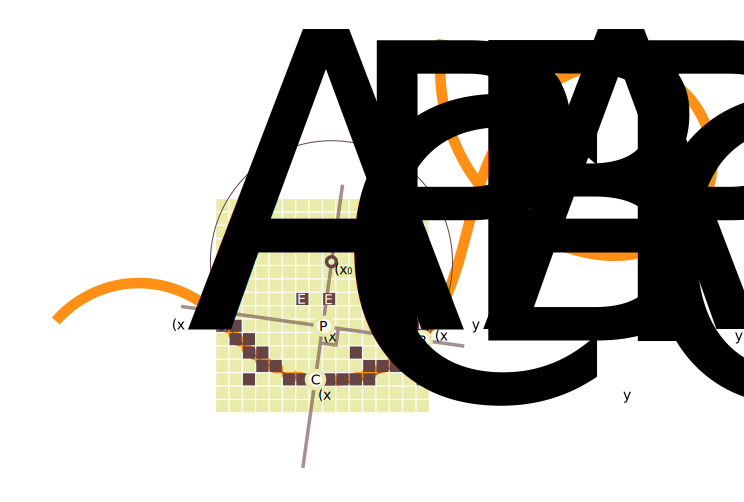
\includegraphics[width=\textwidth]{circle.eps}
\caption{кадр с трассой} \label {fig:search_center:drawings}
\end{figure}

дано $A(x_A \  y_A), B(x_B \  y_B)$

найдём точку $C(x_C \ y_C)$ для этого построим перпендикуляр
посередине отрезка AB. Точка C находится где-то рядом с этим
перпендикуляром (таким образом точки A,B и C будут расположены очень
далеко друг от друга).

Способов нахождения центра окружности $(x_0 \ y_0)$ несколько
(например записать три уравнения $(x_i - x_0)^2 + (y_i - x_0)^2 = R^2$,
 где i=1..3 и решить систему), но у нас уже есть один срединный
перпендикуляр (центр окружности лежит на срединном перпендикуляре
вписанного треугольника), построим второй. Их пересечение и будет
центром окружности.

\subsection{часть первая}
координаты точки P (середины прямой AB):
\begin{equation}
\label{eq:search_center:center_AB}
  x_P = \frac{x_A + x_B}{2} \\
  y_P = \frac{y_A + y_B}{2}
\end{equation}





Уравнение прямой AB (уравнение прямой проходящей через две точки):
\begin{equation}
\label{eq:search_center:line_AB}
\frac{y - y_A}{y_B - y_A} = \frac{x - x_A}{x_B - x_A}
\end{equation}






Если уравнения прямой $y = a_1x+b_1$, где $a_1 = tg(\alpha_1)$ и
$y = a_2x+b_2$, где $a_2 = tg(\alpha_2)$, то прямые перпендикулярны если
$a_1 \cdot a_2 = -1$ и следовательно $a_2 = -\frac{1}{a_1}$


Из уравнения ~\ref{eq:search_center:line_AB} получим
$y = \frac{x - x_A}{x_B - x_A} \cdot (y_B - y_A) + y_A$, и раскрыв скобки:
\begin{equation}
\label{eq:search_center:line_AB_y_ax_b}
y = \underbrace{\frac{y_B - y_A}{x_B - x_A}}_{a_1} \cdot x +  \underbrace{y_A - x_A \cdot \frac{y_B - y_A}{x_B - x_A}}_{b_1}
\end{equation}

значит в уравнении $y = a_2x + b_2$, перпендикулярном уравнению ~\ref{eq:search_center:line_AB_y_ax_b},
коэффициент $a_2 = -\frac{x_B - x_A}{y_B - y_A}$. Осталось найти $b_2$: прямая должна проходить через точку P:

$y_P = a_2x_P + b_2 = -\frac{x_B - x_A}{y_B - y_A} \cdot x_P + b_2$

следовательно $b_2 = y_P + \frac{x_B - x_A}{y_B - y_A} \cdot x_P$

итог:
уравнение прямой P0 перпендикулярное прямой AB (срединный перпендикуляр) выглядит так:

\begin{equation}
\label{eq:search_center:line_P0}
y = -\frac{x_B - x_A}{y_B - y_A} \cdot x + y_P + \frac{x_B - x_A}{y_B - y_A} \cdot x_P
\end{equation}

Проверяем все точки находящиеся на этой прямой или рядом с ней и если они подходят (чёрные) то получаем координаты $C(x_C \  y_C)$.


\subsection{часть вторая}
имея точку A и C повторяем те же действия для построения срединного перпендикуляра между ними:

координаты точки N (середины прямой AC):
\begin{equation}
\label{eq:search_center:center_AC}
  x_N = \frac{x_A + x_C}{2} \\
  y_N = \frac{y_A + y_C}{2}
\end{equation}

пропуская вывод получим уравнение прямой N0 перпендикулярное прямой AC:

\begin{equation}
\label{eq:search_center:line_N0}
y = -\frac{x_C - x_A}{y_C - y_A} \cdot x + y_N - \frac{x_C - x_A}{y_C - y_A} \cdot x_N
\end{equation}

\subsection{часть третья}

две прямые  $y = a_3x+b_3$ и $y = a_4x+b_4$, пересекаются в точке
$x=\frac{b_3-b_4}{a_4-a_3}$
$y=\frac{a_4b_3-a_3b_4}{a_4-a_3}$

наши прямые ~\ref{eq:search_center:line_P0} и ~\ref{eq:search_center:line_N0} выглядят так

\begin{equation}
\label{eq:search_center:line_Y3}
y = \underbrace{-\frac{x_B - x_A}{y_B - y_A}}_{a_3} \cdot x + \underbrace{y_P - \frac{x_B - x_A}{y_B - y_A} \cdot x_P}_{b_3}
\end{equation}

\begin{equation}
\label{eq:search_center:line_Y4}
y = \underbrace{-\frac{x_C - x_A}{y_C - y_A}}_{a_4} \cdot x + \underbrace{y_N - \frac{x_C - x_A}{y_C - y_A} \cdot x_N}_{b_4}
\end{equation}

значит

\begin{equation}
\label{eq:search_center:centerX}
x_0 = \frac{b_3-b_4}{a_4-a_3}
\end{equation}

\begin{equation}
\label{eq:search_center:centerY}
y_0 = \frac{a_4b_3-a_3b_4}{a_4-a_3}
\end{equation}

\subsection{результирующие формулы}

Дано:

$A(x_A \  y_A), B(x_B \  y_B)$

вычисляем:

(уравнение №~\ref{eq:search_center:center_AB}): точку P

$x_P = \frac{x_A + x_B}{2}$

$y_P = \frac{y_A + y_B}{2}$

(уравнение №~\ref{eq:search_center:line_P0}): уравнение прямой для поиска точки C

$y = -\frac{x_B - x_A}{y_B - y_A} \cdot x + y_P + \frac{x_B - x_A}{y_B - y_A} \cdot x_P$

находим точку $C(x_C \  y_C)$

(уравнение №~\ref{eq:search_center:center_AC}) координаты точки N:

$x_N = \frac{x_A + x_C}{2}$ 

$y_N = \frac{y_A + y_C}{2}$



рассчитываем промежуточные коэффициенты

(уравнение №~\ref{eq:search_center:line_Y3}):

$a_3 = -\frac{x_B - x_A}{y_B - y_A}$

$b_3 = y_P - \frac{x_B - x_A}{y_B - y_A} \cdot x_P$

(уравнение №~\ref{eq:search_center:line_Y4}):

$a_4 = -\frac{x_C - x_A}{y_C - y_A}$

$b_4 = y_N - \frac{x_C - x_A}{y_C - y_A} \cdot x_N$

значит координаты центра:

(уравнение №~\ref{eq:search_center:centerX}): $x_0 = \frac{b_3-b_4}{a_4-a_3}$
(уравнение №~\ref{eq:search_center:centerY}): $y_0=\frac{a_4b_3-a_3b_4}{a_4-a_3}$


\end{document}
